\documentclass[hidelinks,12pt,a4paper]{article}

% --- include PDF page ---
\usepackage{pdfpages}

% This doc is used only for combining different title page made with MS word which contains spine.
% It cannot be achieved within the original main.tex file since the original cover page is responsible for aligning all title in the center

% This approach will clear out all of the hyperlink leaving only the text and image behind.

\begin{document}
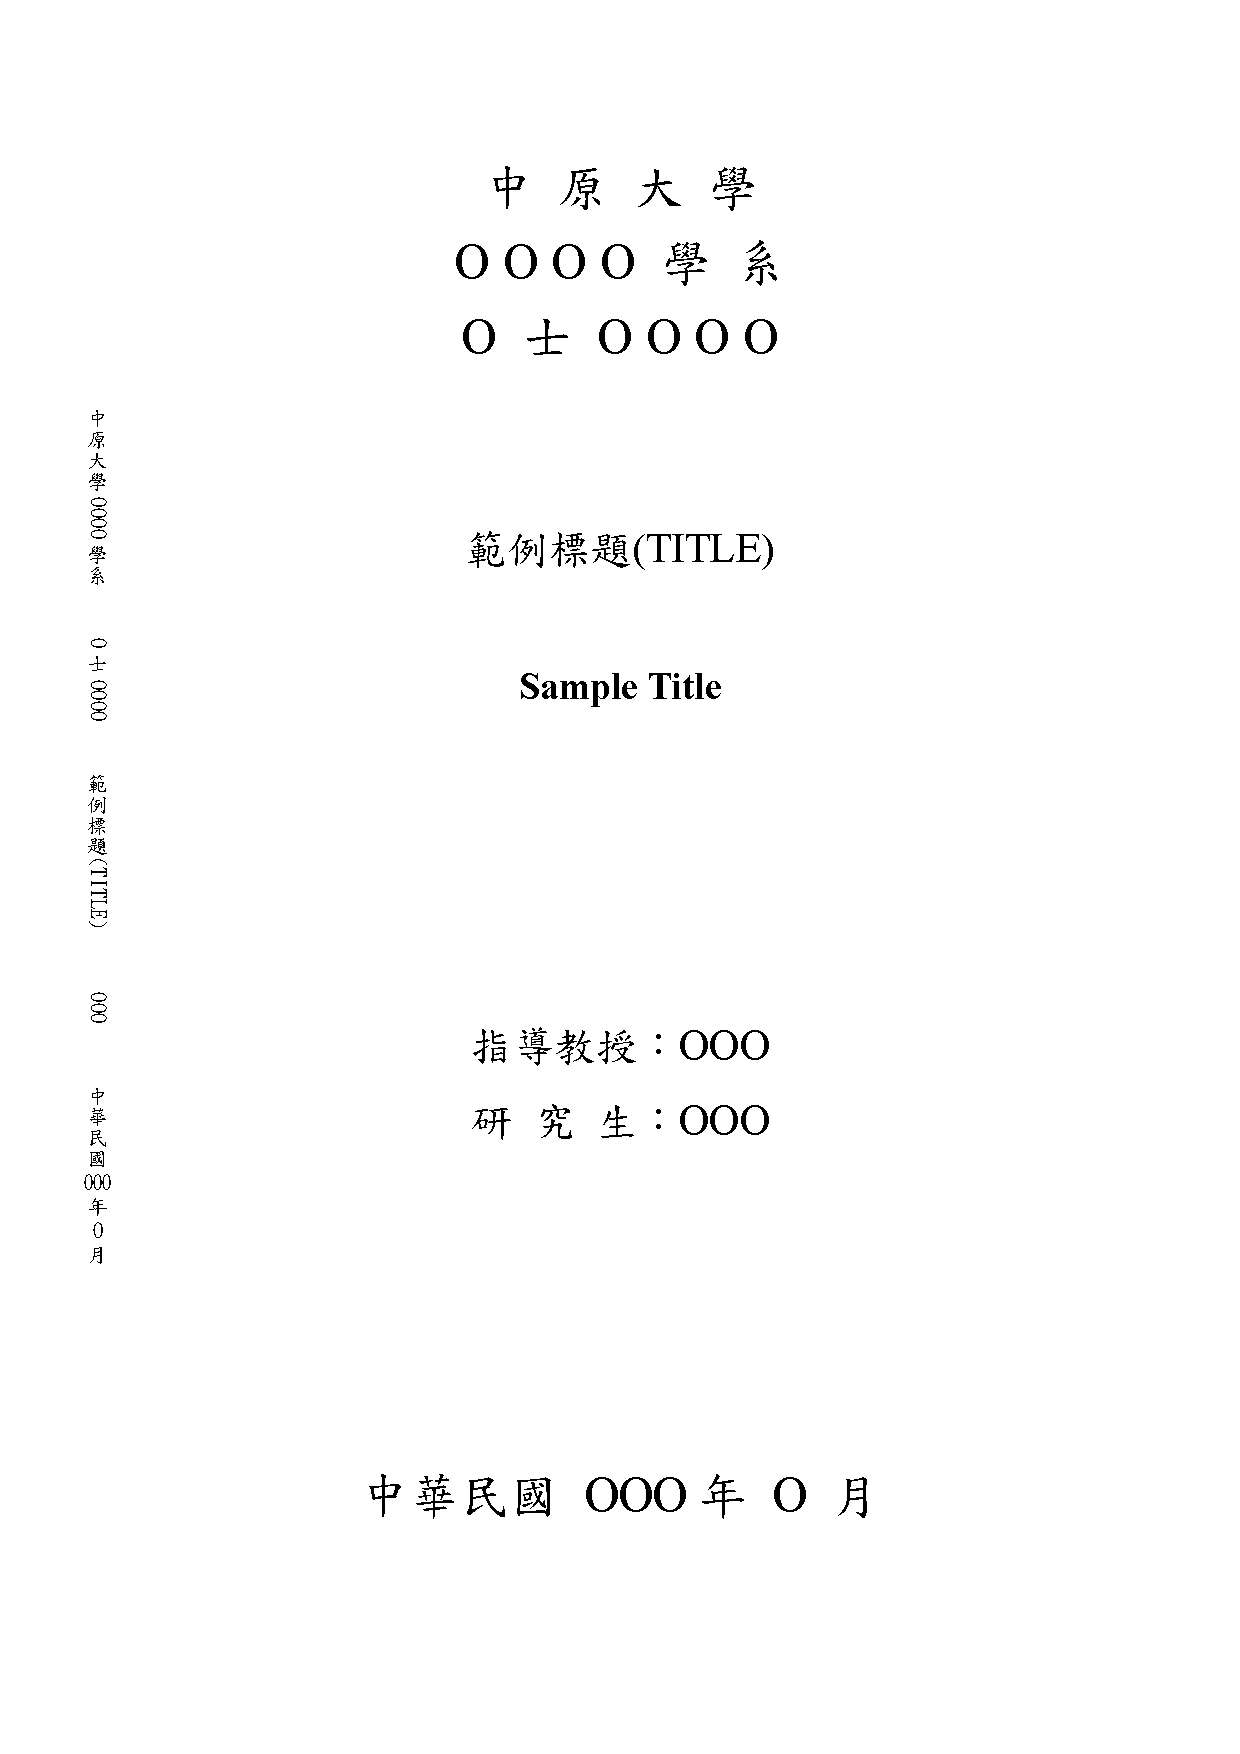
\includepdf[pages=-]{cover_spine.pdf} % title page with spine created by MS word, but this makes all of the title aligned left
\includepdf[pages={2-13}]{main.pdf}
\end{document}
